% Quorum Slice Structure Diagram
% Venn diagram showing tiered quorum structure with infrastructure and community validators
%
% ACCESSIBILITY ALT TEXT:
% A Venn diagram showing Botho's tiered quorum structure. The outer blue
% ellipse contains 4 infrastructure validator nodes (I1-I4) requiring 3-of-4
% agreement. A smaller green ellipse inside contains 3 community validator
% nodes (C1-C3) requiring 2-of-3 agreement. A dashed red outline shows a
% valid quorum that spans both tiers. The design balances stability from
% infrastructure nodes with decentralization from community participation.

\begin{figure}[ht]
\centering
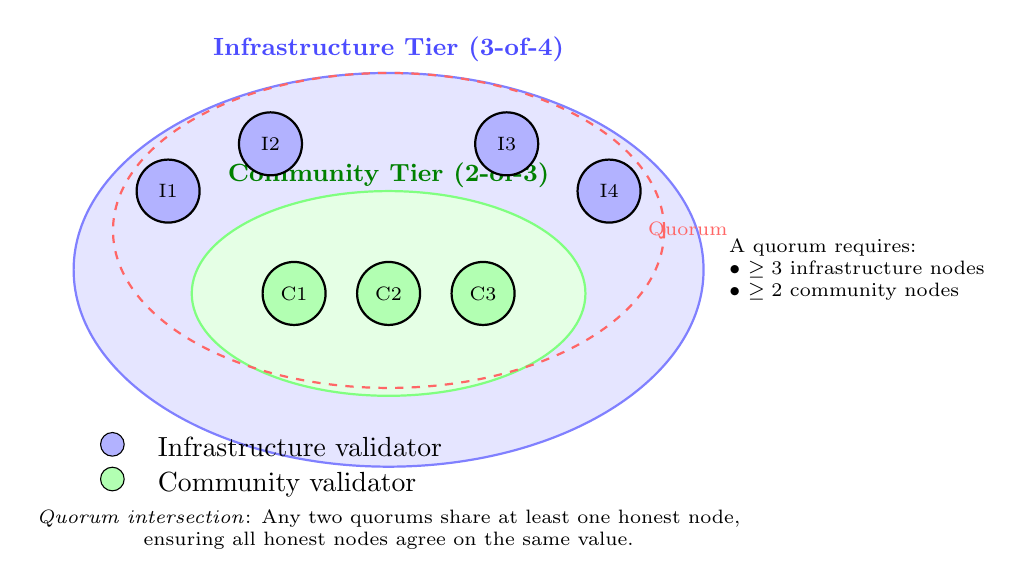
\begin{tikzpicture}[
    node distance=0.8cm,
    validator/.style={circle, draw, minimum size=0.8cm, font=\scriptsize, thick},
    infra/.style={validator, fill=blue!30},
    community/.style={validator, fill=green!30},
    label/.style={font=\small\bfseries},
]

% Infrastructure tier (outer ellipse)
\draw[thick, fill=blue!10, draw=blue!50] (0,0) ellipse (4cm and 2.5cm);
\node[label, blue!70] at (0,2.8) {Infrastructure Tier (3-of-4)};

% Community tier (inner ellipse)
\draw[thick, fill=green!10, draw=green!50] (0,-0.3) ellipse (2.5cm and 1.3cm);
\node[label, green!50!black] at (0,1.2) {Community Tier (2-of-3)};

% Infrastructure nodes
\node[infra] (i1) at (-2.8,1) {I1};
\node[infra] (i2) at (-1.5,1.6) {I2};
\node[infra] (i3) at (1.5,1.6) {I3};
\node[infra] (i4) at (2.8,1) {I4};

% Community nodes
\node[community] (c1) at (-1.2,-0.3) {C1};
\node[community] (c2) at (0,-0.3) {C2};
\node[community] (c3) at (1.2,-0.3) {C3};

% Intersection highlight
\draw[dashed, thick, red!60] (0,0.5) ellipse (3.5cm and 2cm);
\node[font=\scriptsize, red!60] at (3.8,0.5) {Quorum};

% Legend
\node[anchor=west] at (-4,-2.5) {
    \begin{tabular}{ll}
    \tikz\draw[fill=blue!30, draw] (0,0) circle (0.15); & Infrastructure validator \\
    \tikz\draw[fill=green!30, draw] (0,0) circle (0.15); & Community validator \\
    \end{tabular}
};

% Annotations
\node[align=left, font=\scriptsize, anchor=west] at (4.2,0) {
    A quorum requires:\\
    $\bullet$ $\geq 3$ infrastructure nodes\\
    $\bullet$ $\geq 2$ community nodes
};

% Quorum intersection note
\node[align=center, font=\scriptsize] at (0,-3.3) {
    \textit{Quorum intersection}: Any two quorums share at least one honest node,\\
    ensuring all honest nodes agree on the same value.
};

\end{tikzpicture}
\caption{Tiered quorum slice structure in \Botho. Each node's quorum slice requires
agreement from 3-of-4 infrastructure validators AND 2-of-3 community validators.
This design balances network stability (infrastructure tier) with decentralization
(community tier). Quorum intersection is guaranteed when Byzantine nodes are below
threshold.}
\label{fig:quorum-slices}
\end{figure}
